\documentclass[xcolor=tex,dvipsnames]{beamer}  % for hardcopy add 'trans'

\mode<presentation>
{
  \usetheme{Singapore}
  % or ...
  \setbeamercovered{transparent}
  % or whatever (possibly just delete it)
}


\usepackage{fontspec} 
\usepackage[mathscr]{euscript} 
%\usepackage[xcharter]{newtxmath}
%\setmainfont{XCharter}
\setmonofont{DejaVu Sans Mono}[Scale=MatchLowercase] % provides unicode characters 


\usefonttheme{professionalfonts}
%\usepackage[english]{babel}
% or whatever
%\usepackage[latin1]{inputenc}
% or whatever
%\usepackage{times}
\usepackage[T1]{fontenc}
% Or whatever. Note that the encoding and the font should match. If T1
% does not look nice, try deleting the line with the fontenc.

%%%%%%%%%%%%%%%%%%%%%% start my preamble %%%%%%%%%%%%%%%%%%%%%%
\renewcommand{\insertnavigation}[1]{}

\addtobeamertemplate{navigation symbols}{}{%
    \usebeamerfont{footline}%
    \usebeamercolor[fg]{footline}%
    \hspace{1em}%
    \insertframenumber/\inserttotalframenumber
}

\setbeamercolor{footline}{fg=blue}
\setbeamerfont{footline}{series=\bfseries}

%\setbeamertemplate{mini frames}{}

\usepackage{adjustbox}

\usepackage{graphicx}
\usepackage{amsmath, amssymb, amsthm}

\usepackage{fancyvrb}

\usepackage{hyperref}

% fonts, caligraphic
\usepackage{mathpazo}
%\usepackage{mathrsfs}
\usepackage{bbm}

% tikz
\usepackage{tikz}
\usetikzlibrary{positioning}
\usetikzlibrary{arrows}
\usetikzlibrary{calc}
\usetikzlibrary{intersections}
\usetikzlibrary{matrix}
\usetikzlibrary{decorations}
\usepackage{pgf}
\usepackage{pgfplots}
\usetikzlibrary{shapes, fit}

% from fazeleh
\usetikzlibrary{arrows.meta}

%\usetikzlibrary{arrows.meta}
\usetikzlibrary{decorations.pathreplacing}  %for brac



\usepackage{graphviz}

%\usepackage[usenames, dvipsnames]{color}


% nice inequalities
\renewcommand{\leq}{\leqslant}
\renewcommand{\geq}{\geqslant}


\setlength{\parskip}{1.5ex plus0.5ex minus0.5ex}
\setlength{\jot}{12pt} 

\usepackage[ruled, lined]{algorithm2e}


\definecolor{pale}{RGB}{235, 235, 235}
\definecolor{pale2}{RGB}{175,238,238}
\definecolor{turquois4}{RGB}{0,134,139}
\definecolor{DarkOrange1}{RGB}{255,127,0}

\newcommand{\emp}[1]{\textcolor{DarkOrange1}{\bf #1}}
\newcommand{\newtopic}[1]{\textcolor{Green}{\Large \bf #1}}
\newcommand{\navy}[1]{\textcolor{Blue}{\bf #1}}
\newcommand{\navymth}[1]{\textcolor{Blue}{#1}}
\newcommand{\red}[1]{\textcolor{red}{#1}}
\newcommand{\brown}[1]{\textcolor{Brown}{\sf #1}}
\newcommand{\green}[1]{\textcolor{ForestGreen}{\sf #1}}

% Minted
\definecolor{bg}{rgb}{0.95,0.95,0.95}
\usepackage{minted}
\usemintedstyle{friendly}
\newminted{python}{mathescape,frame=lines,framesep=4mm,bgcolor=bg}
\newminted{ipython}{mathescape,frame=lines,framesep=4mm,bgcolor=bg}
\newminted{julia}{mathescape,frame=lines,framesep=4mm,bgcolor=bg}
\newminted{c}{mathescape,frame=lines,framesep=4mm,bgcolor=bg}
\renewcommand{\theFancyVerbLine}{\sffamily
    \textcolor[rgb]{0.5,0.5,1.0}{\scriptsize {\arabic{FancyVerbLine}}}}


\newcommand{\Fact}{\textcolor{Brown}{\bf Fact. }}
\newcommand{\Facts}{\textcolor{Brown}{\bf Facts }}
\newcommand{\keya}{\textcolor{turquois4}{\bf Key Idea. }}
\newcommand{\Factnodot}{\textcolor{Brown}{\bf Fact }}
\newcommand{\Eg}{\textcolor{ForestGreen}{Example. }}
\newcommand{\Egs}{\textcolor{ForestGreen}{Examples. }}
\newcommand{\Ex}{{\bf Ex. }}



\newcommand{\CC}{\mathbbm C}
\newcommand{\EE}{\mathbbm E}
\newcommand{\FF}{\mathbbm F}
\newcommand{\RR}{\mathbbm R}
\newcommand{\KK}{\mathbbm K}
\newcommand{\MM}{\mathbbm M}
\newcommand{\NN}{\mathbbm N}
\newcommand{\PP}{\mathbbm P}
\newcommand{\TT}{\mathbbm T}
\newcommand{\QQ}{\mathbbm Q}
\newcommand{\WW}{\mathbbm W}
\newcommand{\VV}{\mathbbm V}
\newcommand{\ZZ}{\mathbbm Z}

\newcommand{\Asf}{\mathsf A}
\newcommand{\Esf}{\mathsf E}
\newcommand{\Fsf}{\mathsf F}
\newcommand{\Gsf}{\mathsf G}
\newcommand{\Msf}{\mathsf M}
\newcommand{\Lsf}{\mathsf L}
\newcommand{\Nsf}{\mathsf N}
\newcommand{\Psf}{\mathsf P}
\newcommand{\Qsf}{\mathsf Q}
\newcommand{\Ssf}{\mathsf S}
\newcommand{\Tsf}{\mathsf T}
\newcommand{\Xsf}{\mathsf X}
\newcommand{\Ysf}{\mathsf Y}
\newcommand{\Vsf}{\mathsf V}
\newcommand{\Wsf}{\mathsf W}
\newcommand{\Zsf}{\mathsf Z}

\newcommand{\aA}{\mathscr A}
\newcommand{\bB}{\mathscr B}
\newcommand{\cC}{\mathscr C}
\newcommand{\dD}{\mathscr D}
\newcommand{\eE}{\mathscr E}
\newcommand{\gG}{\mathscr G}
\newcommand{\hH}{\mathscr H}
\newcommand{\iI}{\mathscr I}
\newcommand{\fF}{\mathscr F}
\newcommand{\lL}{\mathscr L}
\newcommand{\pP}{\mathscr P}
\newcommand{\rR}{\mathscr R}
\newcommand{\sS}{\mathscr S}
\newcommand{\vV}{\mathscr V}
\newcommand{\wW}{\mathscr W}
\newcommand{\mM}{\mathscr M}
\newcommand{\oO}{\mathscr O}
\newcommand{\zZ}{\mathscr Z}

\newcommand{\bP}{\mathbf P} 
\newcommand{\bR}{\mathbf R}
\newcommand{\bQ}{\mathbf Q}


%%%%%% special symbols %%%%%%%%%%

\newcommand{\volone}{Volume~I}
\newcommand{\voltwo}{Volume~II}

% transpose, not currently using
\newcommand\T{{\mathpalette\raiseT\intercal}}
\newcommand\raiseT[2]{\raisebox{0.25ex}{$#1#2$}}

% nice inequalities
\renewcommand{\leq}{\leqslant}
\renewcommand{\geq}{\geqslant}

% nice greek letters
\renewcommand{\phi}{\varphi}
\renewcommand{\epsilon}{\varepsilon}

% inner product
\providecommand{\inner}[1]{\left\langle{#1}\right\rangle}

% set of matrices
\newcommand{\matset}[2]{ \MM^{ #1 \times #2 } }

% stochastic dominance
\newcommand{\lefsd}{\preceq_{\textrm{F}}}
\newcommand{\lessd}{\preceq_{\textrm{S}}}

% argmax and min
\newcommand{\argmax}{\operatornamewithlimits{argmax}}
\newcommand{\argmin}{\operatornamewithlimits{argmin}}

% sets and logic
\newcommand{\st}{\ensuremath{\ \mathrm{s.t.}\ }}
\newcommand{\setntn}[2]{ \{ #1 : #2 \} }
\newcommand{\natset}[1]{[ #1 ]}

% some useful symbols
\newcommand{\given}{\, | \,}
\newcommand{\cf}[1]{ \lstinline|#1| }
\newcommand{\fore}{\therefore \quad}
\newcommand{\1}{\mathbbm 1}
\newcommand{\me}{\mathrm{e}}               % Euler's e
\newcommand*\diff{\mathop{}\!\mathrm{d}}   % d for integrals

% shortcuts
\newcommand{\la}{\langle}
\newcommand{\ra}{\rangle}

% relations
\newcommand{\eqdist}{\stackrel{d} {=} }
\newcommand{\iidsim}{\stackrel{\textrm{ {\sc iid }}} {\sim} }

% convergence
\newcommand{\tod}{\stackrel { d } {\to} }
\newcommand{\tow}{\stackrel { w } {\to} }
\newcommand{\toprob}{\stackrel { p } {\to} }
\newcommand{\toms}{\stackrel { ms } {\to} }


%%%%%%%%%%% operators %%%%%%%%%%%%

\DeclareMathOperator{\Exp}{Exp}  % exponential draw
\DeclareMathOperator{\Lip}{Lip}
\DeclareMathOperator{\cl}{cl}
\DeclareMathOperator{\graph}{graph}
\DeclareMathOperator{\interior}{int}
\DeclareMathOperator{\Prob}{Prob}
\DeclareMathOperator{\determinant}{det}
\DeclareMathOperator{\trace}{trace}
\DeclareMathOperator{\sgn}{sgn}
\DeclareMathOperator{\Span}{span}
\DeclareMathOperator{\diag}{diag}
\DeclareMathOperator{\proj}{proj}
\DeclareMathOperator{\rank}{rank}
\DeclareMathOperator{\kernel}{null}
\DeclareMathOperator{\cov}{Cov}
\DeclareMathOperator{\corr}{Corr}
\DeclareMathOperator{\var}{Var}
\DeclareMathOperator{\mse}{mse}
\DeclareMathOperator{\se}{se}
\DeclareMathOperator{\range}{range}
\DeclareMathOperator{\dimension}{dim}
\DeclareMathOperator{\epi}{epi}
\DeclareMathOperator{\vecop}{vec}

\DeclareMathOperator{\real}{Re}
\DeclareMathOperator{\imag}{Im}

\DeclareMathOperator{\csum}{cs} % column sum
\DeclareMathOperator{\rsum}{rs} % row sum



\hypersetup{
    linkcolor=Blue,
    colorlinks=true,
    filecolor=magenta,      % color of file links
    urlcolor=cyan           % color of external links
}


%\pgfdeclareimage[height=1.2cm]{university-logo}{../tuxswatter2}
%\logo{\pgfuseimage{university-logo}}

%\addtobeamertemplate{headline}{}
%{%
%\begin{flushright}
%\begin{tikzpicture}[remember picture,overlay]
%\node [left ]{\includegraphics[width=0.5cm]{../tuxswatter2.png}};
%\end{tikzpicture}
%\end{flushright}
%\vskip -0.1cm
%} 

 \date[\today]{}

\title{Quantitative Economics Workshop Paris}







\subtitle{Dynamic Programming}

\author{John Stachurski}

\date{September 2022}


\begin{document}

\begin{frame}
  \titlepage
\end{frame}


\section{Introduction}


\begin{frame}
    \frametitle{Introduction}

    Summary of this lecture:

    \begin{itemize}
        \item Overview of dynamic programming
            \vspace{0.3em}
            \vspace{0.3em}
        \item Introduce RDP framework and provide examples
            \vspace{0.3em}
            \vspace{0.3em}
        \item Provide RDP optimality results
            \vspace{0.3em}
            \vspace{0.3em}
        \item Discuss algorithms
            \vspace{0.3em}
            \vspace{0.3em}
        \item Study their performance for some applications
            \vspace{0.3em}
            \vspace{0.3em}
            \begin{itemize}
                \item optimal savings, optimal investment...
            \end{itemize}
    \end{itemize}

            \vspace{0.3em}
            \vspace{0.3em}

    %\emp{Lecture slides at} \url{https://github.com/jstac/tokyo_2022_coursework}

\end{frame}





\begin{frame}
    \frametitle{Introduction to Dynamic Programming}

    Dynamic program

    \begin{algorithm}[H]
      \DontPrintSemicolon
      an initial state $X_0$ is given \;
      $t \leftarrow 0$ \; %  \tcp{foo}
      \While{$t < T$}
      {
          observe current state $X_t$   \;
          choose action $A_t$ \;
          receive reward $R_t$ based on $(X_t, A_t)$ \;
          state updates to $X_{t+1}$ \;
          $t \leftarrow t + 1$ \;
      }
    \end{algorithm}

\end{frame}

\begin{frame}
    
    \begin{figure}
        \centering
        \vspace{1em}
        \scalebox{0.4}{\input{local_figs/state_action_reward.pdf_t}}
        \vspace{1em}
        \caption{\label{f:state_action_reward} A dynamic program}
    \end{figure}

\end{frame}


\begin{frame}
    
    Comments:
    %
    \begin{itemize}
        \item Objective: maximize \emp{lifetime rewards}
            \vspace{0.3em}
            \vspace{0.3em}
        \begin{itemize}
            \vspace{0.3em}
            \vspace{0.3em}
            \item \Eg $\EE [ R_0 + \beta R_1 + \beta^2 R_2 + \cdots]$ for
                some $\beta \in (0, 1)$
        \end{itemize}
            \vspace{0.3em}
            \vspace{0.3em}
            \vspace{0.3em}
        \item If $T < \infty$ then the problem is called a \navy{finite horizon} problem  
            \vspace{0.3em}
            \vspace{0.3em}
            \vspace{0.3em}
            \vspace{0.3em}
        \item Otherwise it is called an \navy{infinite horizon} problem
    \end{itemize}

\end{frame}


%\begin{frame}

    %\Eg A retailer sets prices and manages inventories to maximize profits

    %\begin{itemize}
        %\item $X_t$ measures 
            %\begin{itemize}
                %\item current business environment
            %\vspace{0.3em}
                %\item the size of the inventories
            %\vspace{0.3em}
                %\item prices set by competitors, etc. 
            %\end{itemize}
            %\vspace{0.3em}
        %\item $A_t$ specifies current prices and orders of new stock
            %\vspace{0.3em}
            %\vspace{0.3em}
        %\item $R_t$ is current profit $\pi_t$
            %\vspace{0.3em}
            %\vspace{0.3em}
        %\item Lifetime reward is 
            %%
            %\begin{equation*}
                %\EE \left[ \pi_0 + \frac{1}{1+r} \pi_1 
                    %+ \left(\frac{1}{1+r}\right)^2 \pi_2
                    %+ \cdots \right]
                    %= \text{EPV}
            %\end{equation*}
    %\end{itemize}


%\end{frame}



\begin{frame}
    \frametitle{Example: Optimal Inventories}

    Given a demand process $(D_t)_{t \geq 0}$, inventory $(X_t)_{t \geq 0}$
    obeys
    %
    \begin{equation*}
        X_{t+1} = F(X_t, A_t, D_{t+1}) 
    \end{equation*}
    %
    where

    \begin{itemize}
        \item the \navy{action} $A_t$ is stock ordered this period 
        \vspace{0.5em}
        \item $F(X, A, D) := \max\{X - D, \, 0\} + A$
    \end{itemize}

    \vspace{0.5em}
    The firm can store at most $K$ items at one time

    \vspace{0.5em}
    \begin{itemize}
        \item The \navy{state space} is $\Xsf := \{0, \ldots, K\}$
    \end{itemize}

    \vspace{0.5em}
    We assume $(D_t) \iidsim \phi \in \dD(\ZZ_+)$  

\end{frame}

\begin{frame}
    
    Profits are 
    %
    \begin{equation*}
        \pi_t := X_t \wedge D_{t+1} - c A_t - \kappa \1\{A_t > 0\}
    \end{equation*}
    %

    \begin{itemize}
        \item sales price $=1$ and orders $>$ inventory are lost 
    \vspace{0.5em}
        \item $c$ is unit product cost 
    \vspace{0.5em}
        \item $\kappa$ is a fixed cost of ordering inventory
    \end{itemize}

    \vspace{0.5em}
    \vspace{0.5em}

    With $\beta := 1/(1+r)$, the value of the firm is 
    %
    \begin{equation*}
        V_0 = \EE \sum_{t \geq 0} \beta^t \pi_t
    \end{equation*}
    %

    \vspace{0.5em}
    \vspace{0.5em}
    Objective: maximize (shareholder) value

\end{frame}


\begin{frame}
    
    Expected current profit is
    %
    \begin{equation*}
        r(x, a)  := \sum_{d \geq 0} (x \wedge d) \phi(d) 
            - c a - \kappa \1\{a > 0\}
    \end{equation*}

    \vspace{0.5em}
    \vspace{0.5em}
    The \navy{feasible correspondence} (which gives feasible order sizes) is
    %
    \begin{equation*}
        \Gamma(x) := \{0, \ldots, K - x\}
    \end{equation*}
    %

    \vspace{0.5em}
    The \navy{Bellman equation} is
    %
    \begin{equation*}
        v(x)
        = \max_{a \in \Gamma(x)} 
        \left\{
            r(x, a)
            + \beta
            \sum_d v[F(x, a, d)] \phi(d)
        \right\}
    \end{equation*}

    The solution $v^*$ equals the value function

\end{frame}

\begin{frame}
    
    The \emp{standard solution procedure} for this problem is VFI:

    \vspace{0.5em}
    \vspace{0.5em}
    %
    \begin{enumerate}
        \item define the \navy{Bellman operator} $T$ via
            %
            \begin{equation*}
                (Tv)(x)
                = \max_{a \in \Gamma(x)} 
                \left\{
                    r(x, a)
                    + \beta
                    \sum_d v[F(x,a,d)] \phi(d)
                \right\}
            \end{equation*}
            \vspace{0.5em}
        \item iterate with $T$ to calculate $v \approx v^*$ and
            \vspace{0.5em}
            \vspace{0.5em}
            \vspace{0.5em}
        \item compute a \navy{$v$-greedy policy} $\sigma^*$, which satisfies
            %
            \begin{equation*}
                \sigma^*(x)
                \in \argmax_{a \in \Gamma(x)} 
                \left\{
                    r(x, a)
                    + \beta
                    \sum_d  v[F(x,a,d)] \phi(d)
                \right\}
            \end{equation*}
    \end{enumerate}

\end{frame}


\begin{frame}
    
    See notebook \texttt{inventory.ipynb}

\end{frame}


\begin{frame}
    \frametitle{Optimal Savings}

    
    Wealth evolves according to
    %
    \begin{equation*}
        C_t + W_{t+1} \leq R W_t + Y_t 
        \qquad (t = 0, 1, \ldots)
    \end{equation*}
    %

        \vspace{0.5em}
    \begin{itemize}
        \item $(W_t)$ takes values in finite set $\Wsf \subset \RR_+$ 
        \vspace{0.5em}
        \item $(Y_t)$ is $Q$-Markov chain on finite set $\Ysf$ 
        \vspace{0.5em}
        \item $C_t \geq 0$
    \end{itemize}

        \vspace{0.5em}
    The household maximizes

    %
    \begin{equation*}
        \EE \sum_{t \geq 0} \beta^t u(C_t)
    \end{equation*}


\end{frame}

\begin{frame}
    
    The Bellman equation is
    %
    \begin{multline*}
        v(w, y) = 
        \\
        \max_{w' \in \Gamma(w, y)}
        \left\{
            u(R w + y - w')
            + \beta \sum_{y' \in \Ysf} v(w', y') Q(y, y')
        \right\}
    \end{multline*}
    %

        \vspace{0.5em}
        \vspace{0.5em}
    The standard solution procedure is VFI

    \begin{enumerate}
        \item Set up Bellman operator $T$
        \vspace{0.5em}
        \item Iterate with $T$ from some initial guess to approximate $v^*$
        \vspace{0.5em}
        \item Compute the $v^*$-greedy policy
    \end{enumerate}

\end{frame}



\begin{frame}
    \frametitle{Recursive Decision Processes}

    We will study an abstract dynamic program with Bellman equation
    %
    \begin{equation*}
        v(x) = \max_{a \in \Gamma(x)} B(x, a, v)
    \end{equation*}

        \vspace{0.5em}
        \vspace{0.5em}
    Advantages of ``abstract'' dynamic programming

    \begin{itemize}
        \item Subsumes standard Markov decision processes
        \vspace{0.5em}
        \item Can handle state-dependent discounting, recursive prefs, etc.
        \vspace{0.5em}
        \item Abstraction means clean proofs
        \vspace{0.5em}
        \item Abstraction allows better analysis of algorithms
    \end{itemize}

\end{frame}


\begin{frame}
    
    Let $\Xsf$ and $\Asf$ be finite sets (\navy{state} and \navy{action spaces})

        \vspace{0.5em}
    Actions are constrained by the \navy{feasible correspondence} ---
        a nonempty correspondence $\Gamma$ from $\Xsf$ to $\Asf$ 
            

        \vspace{0.5em}

    The feasible correspondence in turn defines
    %
    \begin{enumerate}
        \item the \navy{feasible state-action pairs}
            %
            \begin{equation*}
                \Gsf := \setntn{(x, a) \in \Xsf \times \Asf}{a \in \Gamma(x)}
            \end{equation*}
            %
        \item the set of \navy{feasible policies} 
            %
            \begin{equation*}
                \Sigma := 
                    \setntn{\sigma \in \Asf^\Xsf}
                    {\sigma(x) \in \Gamma(x) \text{ for all } x \in \Xsf}.
            \end{equation*}
            %
    \end{enumerate}

    \begin{itemize}
        \item ``follow'' $\sigma$ $\iff$ always respond to state $x$ with action
            $\sigma(x)$
    \end{itemize}

\end{frame}

\begin{frame}
    
    Given $\Xsf$, $\Asf$ and $\Gamma$, a \navy{recursive
    decision process} (RDP) consists of
    %
    
        \vspace{0.5em}
    \begin{enumerate}
        \item a subset $\vV$ of $\RR^\Xsf$ called the 
            \navy{candidate value functions} and
        \vspace{0.5em}
        \vspace{0.5em}
        \item a \navy{value aggregator}, which is a function
                %
                \begin{equation*}
                    B \colon \Gsf \times \vV \to \RR
                \end{equation*}
                %
              satisfying $v, w \in \vV$ and $v \leq w \implies$
              %
              \vspace{0.5em}
              \begin{equation*}
                B(x, a, v) \leq B(x, a, w) \; \text{ for all $(x, a) \in \Gsf$}
              \end{equation*}
                %
              and 
                %
                \begin{equation*}
                    \sigma \in \Sigma 
                    \, \text{ and } \,
                    v \in \vV
                    \; \implies \;
                    w \in \vV
                    \quad \text{ where }
                    w(x) := B(x, \sigma(x), v)
                \end{equation*}
                %
    \end{enumerate}

\end{frame}


\begin{frame}
    

    \Eg For the inventory problem we set 
    %
    \begin{itemize}
        \item $\Gamma(x) := \{0, \ldots, K - x\}$
        \vspace{0.3em}
        \item $\vV = \RR^\Xsf$ and
        %
        \begin{equation*}
            B(x, a, v) :=
                r(x, a)
                + \beta
                \sum_{d \geq 0} v[F(x,a,d)] \phi(d)
        \end{equation*}
    \end{itemize}

    The Bellman equation is then 
    %
    $$v(x) = \max_{a \in \Gamma(x)} B(x, a, v)$$

    The function $B$ is a valid aggregator

        \vspace{0.3em}
    For example, if $v \leq w$, then
    %
    \begin{equation*}
        B(x, a, v) \leq B(x, a, w)
    \end{equation*}

\end{frame}


\begin{frame}
    

    \Eg For the savings problem we set 
    %
    \begin{itemize}
        \item $\Gamma(w, y) := \{w' \in \Wsf \,:\, w' \leq Rw + y\}$
        \vspace{0.3em}
        \item $\vV = \RR^\Xsf$ and
        %
        \begin{equation*}
            B((w,y), w', v) :=
            u(R w + y - w')
            + \beta \sum_{y' \in \Ysf} v(w', y') Q(y, y')
        \end{equation*}
    \end{itemize}

    The Bellman equation is then 
    %
    $$v(w, y) = \max_{w' \in \Gamma(w, y)} B((w, y), w', v)$$

    The function $B$ is a valid aggergator

        \vspace{0.3em}
    For example, if $f \leq g$, then
    %
    \begin{equation*}
        B((w,y), w', f) \leq B((w,y), w', g)
    \end{equation*}

\end{frame}


\begin{frame}
    
    The RDP framework admits a huge range of generalizations

              \vspace{0.5em}
              \vspace{0.5em}
    \Eg State-dependent discounting: replace $\beta$ with 
    %
    \begin{equation*}
        \beta_t = \beta(Z_t)  \text{ where $Z_t$ is a new state variable}
    \end{equation*}

              \vspace{0.5em}
              \vspace{0.5em}
    \Eg Epstein--Zin preferences:
    %
    \begin{equation*}
        B(x, a, v) =
        \left\{
            r(x, a)^\alpha + \beta 
                \left[
                    \sum_{x' \in \Xsf} v(x')^\gamma P(x,a, x')
                \right]^{\alpha / \gamma}
        \right\}^{1/\alpha}
    \end{equation*}

              \vspace{0.5em}
    \Eg Risk-sensitive preferences, ambiguity aversion, shortest path problems, etc.
     
\end{frame}


\begin{frame}
    \frametitle{Lifetime Value}

    Fix $\sigma \in \Sigma$ 

              \vspace{0.5em}
              \vspace{0.5em}
    A $v \in \vV$ that satisfies
    %
    \begin{equation*}
        v(x) = B(x, \sigma(x), v)
        \quad \text{for all } x \in \Xsf
    \end{equation*}
    %
    is called a \navy{$\sigma$-value function}

              \vspace{0.5em}
              \vspace{0.5em}
    \emp{Key idea:} a $\sigma$-value function gives the \underline{lifetime
    value} of following $\sigma$, from each state

              \vspace{0.5em}
              \vspace{0.5em}

    Why is this interpretation valid?

\end{frame}

\begin{frame}
    
    \Eg In the inventory problem, a $\sigma$-value function solves 
    %
    \begin{equation*}
        v(x)
        = r(x, \sigma(x))
                + \beta
                \sum_d v [F(x, \sigma(x), d) ] \phi(d)
    \end{equation*}

              \vspace{0.5em}
    With a change of variable, we can write this as
    %
    \begin{equation*}
        v(x)
        = r(x, \sigma(x))
                + \beta
                \sum_{x'} v (x') P(x, \sigma(x), x') 
    \end{equation*}

    where
    %
    \begin{equation*}
        P(x, a, x') := \PP\{ F(x,a,D) = x' \}
        \quad \text{when} \quad
        D \sim \phi
    \end{equation*}

              \vspace{0.5em}
    In matrix notation,
    %
    \begin{equation*}
        v = r_\sigma + \beta \, P_\sigma \, v
    \end{equation*}

\end{frame}

\begin{frame}
    
    Solving this equation gives the $\sigma$-value function:
    %
    \begin{equation*}
        v_\sigma = (I - \beta P_\sigma)^{-1} r_\sigma
    \end{equation*}

              \vspace{0.5em}
              \vspace{0.5em}
    Applying the Neumann series lemma, we can write $v_\sigma$ as
    %
    \begin{equation*}
        v_\sigma = \sum_{t \geq 0} \beta^t P_\sigma^t r_\sigma
    \end{equation*}

              \vspace{0.5em}
              \vspace{0.5em}
    This is the lifetime value of the profit flow when 
    %
    \begin{itemize}
        \item following policy $\sigma$
              \vspace{0.5em}
        \item discounting at rate $\beta$
    \end{itemize}

\end{frame}

\begin{frame}

    Now let's return to the general case, with RDP $(\Gamma, \vV, B)$

        \vspace{0.5em}
        \vspace{0.5em}
    Is lifetime value well-defined?
        \vspace{0.5em}
        \vspace{0.5em}

    To answer this we introduce the \navy{policy operator} $T_\sigma$ via
    %
    \begin{equation*}
        (T_\sigma \, v)(x) = B(x, \sigma(x), v)
        \qquad (x \in \Xsf,\; v \in \vV)
    \end{equation*}
    %

    \emp{Note:} $v \in \vV$ is a $\sigma$-valued function iff $v$ is a fixed point of
    $T_\sigma$
    
        \vspace{0.5em}
        \vspace{0.5em}

    Below we impose conditions under which $T_\sigma$ always has a unique
    fixed point, \navy{denoted by $v_\sigma$}

        \vspace{0.5em}
        \vspace{0.5em}
    Hence lifetime value is always uniquely defined


\end{frame}


\begin{frame}
    
    With lifetime value uniquely defined for each $\sigma$, we can discuss
    optimality

        \vspace{0.5em}
        \vspace{0.5em}
    A policy $\sigma^* \in \Sigma$ is called \navy{optimal} if
    %
    \begin{equation*}
        v_{\sigma^*}(x) = \max_{\sigma \in \Sigma} v_\sigma(x)
        \quad \text{for all } x \in \Xsf
    \end{equation*}

        \vspace{0.5em}
        \vspace{0.5em}
    Also, the \navy{value function} is defined as 
    %
    \begin{equation*}
        v^*(x) = \max_{\sigma \in \Sigma} v_\sigma(x)
        \quad (x \in \Xsf)
    \end{equation*}

        \vspace{0.5em}
        \vspace{0.5em}
    Hence $\sigma^*$ is optimal iff $v_{\sigma^*} = v^*$

        \vspace{0.5em}
        \vspace{0.5em}

    But \underline{how do we find optimal policies}??

\end{frame}


\begin{frame}
    \frametitle{Operators}

    Given $v$ in $\vV$, we call $\sigma \in \Sigma$ \navy{$v$-greedy}  if 
    %
    \begin{equation*}
        \sigma(x) \in \argmax_{a \in \Gamma(x)} B(x, a, v)
        \qquad \text{for all } x \in \Xsf
    \end{equation*}
    %

              \vspace{0.5em}
    The \navy{Bellman operator} is defined by
    %
    \begin{equation*}
        (T v)(x) = \max_{a \in \Gamma(x)} B(x, a, v)
        \qquad (x \in \Xsf, \; v \in \vV)
    \end{equation*}
    %

          \vspace{0.5em}

    Notes:
    %
    \begin{itemize}
        \item $v$ solves the Bellman equation iff $v$ is a fixed point of $T$
          \vspace{0.5em}
        \item $(Tv)(x) = \max_{\sigma \in \Sigma} (T_\sigma \, v)(x)$
    \end{itemize}


\end{frame}


\begin{frame}
    \frametitle{Stability}
    
    Let $\rR := (\Gamma, \vV, B)$ be an RDP with 
    %
    \begin{itemize}
        \item Bellman operator $T$ and 
        \item policy operators $\{T_\sigma\}_{\sigma \in \Sigma}$
    \end{itemize}


        \vspace{0.5em}
        \vspace{0.5em}
        \vspace{0.5em}
    We call $\rR$ \navy{globally stable} if
    %
    \begin{enumerate}
        \item $T$ is globally stable on $\vV$ and
        \vspace{0.5em}
        \item $T_\sigma$ is globally stable on $\vV$ for all $\sigma \in \Sigma$
    \end{enumerate}

\end{frame}


\begin{frame}
    
    \Eg In the inventory problem, the operator $T_\sigma$ is defined by 
    %
    \begin{equation*}
        (T_\sigma v)(x)
        = r(x, \sigma(x))
                + \beta
                \sum_d v [F(x, \sigma(x), d) ] \phi(d)
    \end{equation*}

    Hence, fixing $x \in \Xsf$ and $v, w \in \vV$,
    %
    \begin{multline*}
        |(T_\sigma v)(x) -(T_\sigma w)(x)|
        \\ 
        =
        \beta \,
        \left| 
            \sum_d v [F(x, \sigma(x), d) ] \phi(d)
            - \sum_d w [F(x, \sigma(x), d) ] \phi(d)
        \right|
    \end{multline*}
    %
    This is bounded above by 
    %
    \begin{align*}
        \beta \,
        \sum_d
        \left| 
            v [F(x, \sigma(x), d) ]
            -w [F(x, \sigma(x), d) ]
        \right| \phi(d)
        \leq \beta \| v - w\|_\infty
    \end{align*}
    %

\end{frame}


\begin{frame}

    In summary,
    %
    \begin{equation*}
        |(T_\sigma v)(x) -(T_\sigma w)(x)|
        \leq \beta \| v - w\|_\infty
        \quad \text{for all } x \in \Xsf
    \end{equation*}
    
        \vspace{0.5em}
    Taking the max over $x$ gives
    %
    \begin{equation*}
        \|T_\sigma v -T_\sigma w \|_\infty
        \leq \beta \| v - w\|_\infty
        \quad \text{for all } x \in \Xsf
    \end{equation*}


        \vspace{0.5em}
    Hence $T_\sigma$ is a contraction on $\vV = \RR^\Xsf$

        \vspace{0.5em}
    In particular, $T_\sigma$ is globally stable on $\vV$

        \vspace{0.5em}
        \vspace{0.5em}
    A similar argument works for $T$

\end{frame}


\begin{frame}

    Which other DP problems are globally stable?

        \vspace{0.5em}
    \begin{itemize}
        \item the optimal savings problem
            \vspace{0.5em}
        \item all standard Markov decision problems
            \vspace{0.5em}
        \item models with time-varying discount rates, under certain
            conditions
            \vspace{0.5em}
        \item models with risk-sensitive preferences, under some conditions
            \vspace{0.5em}
        \item models with Epstein--Zin preferences, under some conditions
            \vspace{0.5em}
        \item etc.
    \end{itemize}
    

\end{frame}



\begin{frame}
    

    {\bf Theorem.} For every globally stable RDP, the following statements are true:
    %
    \begin{enumerate}
        \item The value function $v^*$ satisfies the Bellman equation
            \vspace{1em}
        \item $v^*$ is the only fixed point of $T$ in
            $\vV$ and 
            %
            \begin{equation*}
                \lim_{k \to \infty} T^k v = v^*
                \quad \text{for all } v \in \vV
            \end{equation*}
            %
        \item A policy $\sigma \in \Sigma$ is optimal if and only if it is
            $v^*$-greedy
            \vspace{1em}
        \item At least one optimal policy exists
    \end{enumerate}
    %

\end{frame}



\begin{frame}
    
    \begin{figure}
        \centering
        \scalebox{0.6}{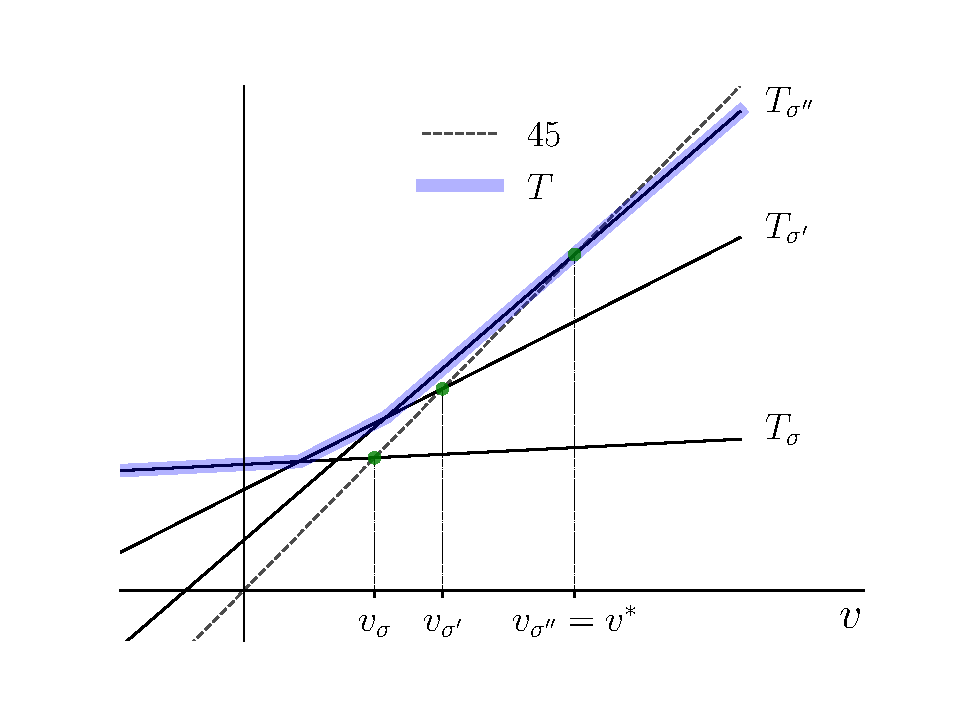
\includegraphics{local_figs/optimality_illustration_1.pdf}}
        \caption{1D case when $T_\sigma \, v = r_\sigma + \beta P_\sigma \, v$ and $\Sigma = \{\sigma, \sigma', \sigma''\}$}
    \end{figure}
    %



\end{frame}


\begin{frame}
    \frametitle{Algorithms}

    We used VFI to solve some simple problems

    \vspace{0.5em}
    \vspace{0.5em}
    Next we
    %
    \begin{enumerate}
        \item present a generalization of VFI suitable for aribtrary RDPs
    \vspace{0.5em}
        \item introduce two other important methods
    \end{enumerate}

    \vspace{0.5em}
    The two other methods are called
    %
    \begin{enumerate}
        \item Howard policy iteration (HPI) and
    \vspace{0.5em}
        \item Optimistic policy iteration (OPI)
    \end{enumerate}


\end{frame}


\begin{frame}
    
{\small 
    \begin{algorithm}[H]
    \DontPrintSemicolon
    input $v_0 \in \RR^\Xsf$, an initial guess of $v^*$ \;
    input $\tau$, a tolerance level for error \;
    $\epsilon \leftarrow \tau + 1$ \;
    $k \leftarrow 0$ \;
    \While{$\epsilon > \tau $}
    {
        \For{$x \in \Xsf$}
        {
            $v_{k+1}(x) \leftarrow (Tv_k) (x)$ \;
        }
        $\epsilon \leftarrow \| v_k - v_{k+1} \|_\infty$ \;
        $k \leftarrow k + 1$ \;
    }
    Compute a $v_k$-greedy policy $\sigma$ \;
    \Return{$\sigma$}
    \caption{VFI for RDPs}
    \end{algorithm}
}

\end{frame}

\begin{frame}
    

    VFI is 
    %
    \begin{itemize}
        \item robust
        \vspace{0.5em}
        \item easy to implement 
        \vspace{0.5em}
        \item very popular in economics (almost universal)
    \end{itemize}

    \vspace{0.5em}
    \vspace{0.5em}
    \vspace{0.5em}
    However, 
    %
    \begin{itemize}
        \item we can often find faster methods 
        \vspace{0.5em}
        \item VFI is relatively serial  --- can be hard to parallelize efficiently
    \end{itemize}

\end{frame}


\begin{frame}
    \frametitle{Howard Policy Iteration}

    \begin{figure}
       \begin{center}
           \scalebox{0.7}{
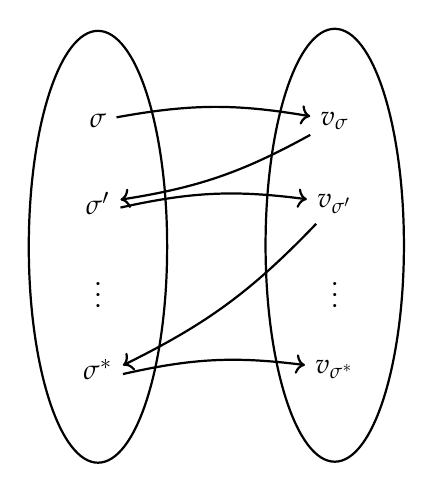
\begin{tikzpicture}[auto, thick, node distance=30pt, bend left=10]

\node (s) {$\sigma$};
\node (s1) [below of=s] {$\sigma'$};
\node (el1) [below of=s1] {$\vdots$};
\node (s2) [below of=el1] {$\sigma^*$};

\node (v) [right=70pt of s] {$v_{\sigma}$};
\node (v1) [below of=v] {$v_{\sigma'}$};
\node (el2) [below of=v1] {$\vdots$};
\node (v2) [below of=el2] {$v_{\sigma^*}$};

\node[draw, ellipse, minimum width=50pt, fit=(s) (s1) (s2)](f1) {};
\node[draw, ellipse, minimum width=50pt, fit=(v) (v1) (v2)](f2) {};

\draw[->] (s) to (v);
\draw[->] (v) to (s1.10);
\draw[->] (s1.-10) to (v1);
\draw[->] (v1) to (s2.10);
\draw[->] (s2.-10) to (v2);

\end{tikzpicture}
}
        \vspace{1em}
       \end{center}
    \end{figure}

    Iterates between computing the value of a given policy
    and computing the greedy policy associated with that value

\end{frame}

\begin{frame}
        
    {\small
    \begin{algorithm}[H]
        \DontPrintSemicolon
        input $\sigma_0 \in \Sigma$, an initial guess of $\sigma^*$ \;
        $k \leftarrow 0$ \;
        $\epsilon \leftarrow 1$ \;
        \While{$\epsilon > 0 $}
        {
            $v_k \leftarrow $ the $\sigma_k$-value function \;
            $\sigma_{k+1} \leftarrow $ a $v_k$ greedy policy \;
            $\epsilon \leftarrow \| \sigma_k - \sigma_{k+1} \|_\infty$ \;
            $k \leftarrow k + 1$ \;
        }
        \Return{$\sigma_k$}
        \caption{\label{algo:fshpi} Howard policy iteration (HPI) for RDPs}
    \end{algorithm}
    }

        \vspace{1em}
        \vspace{1em}
    \begin{itemize}
        \item In fact this is Newton's algorithm applied to $T$!
    \end{itemize}

\end{frame}

\begin{frame}
    
    Advantages:
    %
    \begin{enumerate}
        \item in a finite state setting, HPI always converges to the
            \underline{exact} optimal policy in a \underline{finite} number of steps
        \vspace{0.5em}
        \item the rate of convergence is faster that VFI 
    \end{enumerate}


        \vspace{0.5em}
      But 
      %
      \begin{itemize}
          \item exact computation of the value of each policy can be
              problematic
          \item faster rate but the constant can be larger than VFI\ldots
      \end{itemize}


\end{frame}


\begin{frame}
    \frametitle{Optimistic Policy Iteration}

    OPI borrows from both value function iteration and Howard policy iteration

    \vspace{0.5em}
    The same as Howard policy iteration (HPI) except that
    %
    \begin{itemize}
        \item HPI takes $\sigma$ and obtains $v_\sigma$
    \vspace{0.5em}
        \item OPI takes $\sigma$ and iterates $m$ times with $T_{\sigma}$
    \end{itemize}


    \vspace{0.5em}
    Recall that $T^m_{\sigma} \to v_\sigma$ as $m \to \infty$

    \vspace{0.5em}
    \vspace{0.5em}
    Hence OPI replaces $v_\sigma$ with an approximation

\end{frame}


\begin{frame}
    
    {\small
    \begin{algorithm}[H]
        \DontPrintSemicolon
        input $v_0 \in \RR^\Xsf$, an initial guess of $v^*$ \;
        input $\tau$, a tolerance level for error \;
        input $m \in \NN$, a step size \;
        $k \leftarrow 0$ \;
        $\epsilon \leftarrow \tau + 1$ \;
        \While{$\epsilon > \tau $}
        {
            $\sigma_k \leftarrow $ a $v_k$-greedy policy \;
            $v_{k+1} \leftarrow T_{\sigma_k}^m v_k$  \;
            $\epsilon \leftarrow \| v_k - v_{k+1} \|_\infty$ \;
            $k \leftarrow k + 1$ \;
        }
        \Return{$\sigma_k$}
        \caption{Optimistic policy iteration for RDPs}
    \end{algorithm}
    }

\end{frame}


\begin{frame}
    

    Under mild conditions, $(\sigma_k)_{k \geq 1}$ converges to an optimal policy
    \vspace{0.5em}
    \vspace{0.5em}

    Regarding $m$,
    %
    \begin{itemize}
        \item $m=\infty \, \implies$ OPI $=$ HPI
    \vspace{0.5em}
        \item $m=1 \, \implies$ OPI $=$ VFI
    \end{itemize}

    \vspace{0.5em}
    \vspace{0.5em}
    \vspace{0.5em}
    Often an intermediate value of $m$ is better than both


\end{frame}

\begin{frame}
    
    We investigate efficiency of VFI--HPI--OPI in two applications 

    \vspace{0.5em}
    \begin{itemize}
        \item \texttt{investment.ipynb}
    \vspace{0.5em}
        \item \texttt{opt\_savings.ipynb}
    \end{itemize}

\end{frame}



\end{document}









